\newpage
\section{Aufgabenstellung 3}

%\subsection{Ausgangssituation}
%Sie sind Teil eines Qualitätssicherungsteams in einem fiktiven Unternehmen, das eine E-Commerce-Plattform betreibt. Die Plattform bietet Kameraprodukte an, nutzt KI-gestützte Produktsuche, integriert verschiedene Backend-Systeme (z. B. SAP, AWS, NetSuite, HubSpot) und führt den Nutzer durch einen komplexen, serviceorientierten Kaufprozess.Ein zentraler Bestandteil dieses Systems ist der in der beigefügten Prozessgrafik dargestellte End-to-End-Ablauf, vom Website-Besuch bis zur finalen Mail-Bestätigung. Die Architektur umfasst APIs, externe Services, Cloud-Provisionierung und ERP-Integration.

%\subsection{Ziel}
%\textit{Erarbeiten Sie als Gruppe eine ganzheitliche Teststrategie für dieses System. Die Strategie soll praktikabel sein, typische Herausforderungen im DevOps-Umfeld adressieren und die Integration verschiedener Testebenen, Tools und Umgebungen berücksichtigen.}

%\subsection{Bearbeitungsschwerpunkte}
%\textit{Bitte erarbeiten Sie eine Ausarbeitung (max. 6 Seiten + Anhang), in der Sie folgende Punkte behandeln:}

\subsection{Testumgebungsstabilisierung}
%\begin{itemize}
%    \item \textit{Wie stellen Sie in der Entwicklungs- und Integrationsphase eine stabile Testumgebung sicher, insbesondere angesichts externer Systeme (SAP, AWS, GPT, HubSpot etc.)?}
%    \item \textit{Wie kann Service-Virtualisierung oder Mocking zum Einsatz kommen?}
%    \item \textit{Welche Datenanforderungen bestehen (z. B. synthetische Testdaten, Daten-Maskierung)?}
%\end{itemize}
Für unsere E-Commerce-Plattform mit ihren vielfältigen Integrationen (SAP, AWS, GPT, HubSpot) setzen wir auf:
\begin{itemize}
    \item \textbf{Infrastruktur als Code (IaC):} Wir nutzen Terraform/CloudFormation, um isolierte Testumgebungen automatisiert zu erstellen und zu verwalten.
    \item \textbf{Umgebungsmodellierung:} Jede Testumgebung wird mit ihren Komponenten, Konfigurationen und Testdaten dokumentiert, für bessere Transparenz und Kontrolle.
    \item \textbf{Containerisierung:} Kubernetes-Namespaces für kurzlebige, isolierte Testumgebungen.
    \item \textbf{Sandbox-Accounts:} Dedizierte Test-Accounts für Cloud-Dienste verhindern Konflikte zwischen Teams.
\end{itemize}
Zusammenfassend isolieren wir und verwalten die Infrastruktur mittels Infrastructure as Code (z.\,B. Terraform/CloudFormation) und nutzen dedizierte Sandbox-Accounts, um Konflikte zu vermeiden. Service-Virtualisierung ist eine zentrale Strategie die im nächsten Abschnitt beschrieben wird. Für eine beispielhafte Darstellung der Umgebung siehe Abbildung~\ref{fig:deployment}).
\begin{figure}[h!]
\centering
\caption{Deployment-Diagramm: Virtuelle Testumgebungen via IaC}
    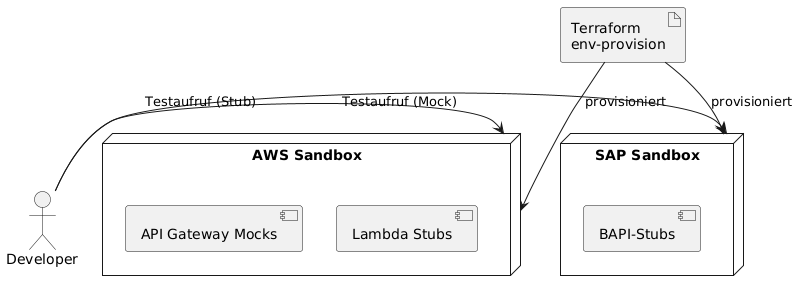
\includegraphics[width=0.8\textwidth]{fig/stubing.png}
    \label{fig:deployment}
\end{figure}
\subsubsection{Service-Virtualisierung und Mock-Ansätze}
Service-Virtualisierung ist entscheidend, wenn externe Systeme nicht verfügbar oder instabil sind:
\begin{itemize}
    \item \textbf{REST/HTTP-Interfaces:} WireMock oder Mountebank für die Simulation von REST-APIs \cite{wiremock2025}.
    \item \textbf{Cloud-APIs:} AWS LocalStack für lokale Emulation von AWS-Services \cite{aws2021}.
    \item \textbf{ERP-Integration:} Virtualisierung von SAP BAPIs und speziellen Schnittstellen.
    \item \textbf{API-Gateway:} Nutzung von AWS API Gateway zur Erstellung von Mock-Endpunkten.
\end{itemize}
Wenn abhängige Systeme (ERP oder externe APIs) instabil oder nicht verfügbar sind, simulieren Virtualisierungstools realistische Interaktionen. Open-Source-Lösungen wie WireMock oder Mountebank (siehe dazu \citet{byars2018}) stubben REST-/HTTP-Schnittstellen, während Cloud-Tools (z.\,B. AWS LocalStack) Cloud-APIs lokal emulieren. Der Ablauf ist in Abbildung~\ref{fig:sequence} dargestellt.\begin{figure}[h!]
\centering
\caption{Sequenzdiagramm: Service-Virtualisierung mit WireMock}
    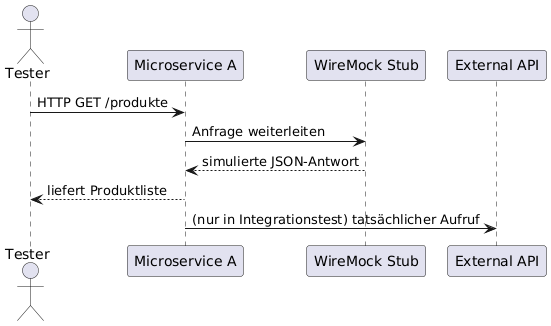
\includegraphics[width=0.8\textwidth]{fig/servicevirti.png}
    \label{fig:sequence}
\end{figure}

\newpage
\subsubsection{Testdatenmanagement}
Um konsistente und compliance-konforme Tests zu gewährleisten:
\begin{itemize}
    \item \textbf{Datenmaskierung:} Ersetzen von PII mit realistischen fiktiven Werten unter Beibehaltung der referentiellen Integrität.\citet{tricentis2024} empfiehlt Format-preserving Encryption für PII
    \item \textbf{Synthetische Daten:} Künstliche Datensätze für Spezialfälle und Randszenarien.\citet{browserstack2025} kombiniert synthetische und maskierte Daten
    \item \textbf{Hybridansatz:} Maskierte Produktionsdaten für Basistests, ergänzt durch synthetische Daten für Edge-Cases.
    \item \textbf{API-Integration:} CI/CD-Pipeline kann Testdaten über APIs auffrischen, zurücksetzen oder klonen.
\end{itemize}
\subsection{2. Testarten und Abdeckung}
%\begin{itemize}
%    \item \textit{Welche Testarten (z. B. Unit-, API-, Integrations-, E2E-, Load-, Performance-, Security-tests) sind erforderlich, um:}
%    \begin{itemize}
%        \item \textit{die funktionalen Anforderungen abzudecken?}
%        \item \textit{nicht-funktionale Anforderungen wie Performance, Security, Verfügbarkeit und Datenintegrität zu prüfen?}
%    \end{itemize}
%    \item \textit{Wo und wie werden diese Tests innerhalb der CI/CD-Pipeline ausgeführt?}
%\end{itemize}

\subsubsection{Funktionale Tests}
Zur Abdeckung funktionaler Anforderungen setzen wir folgende Testtypen ein:
\begin{itemize}
    \item \textbf{Unit-Tests:} Für einzelne Module/Services, laufen bei jedem Commit.
    \item \textbf{API-Tests:} Validierung jeder Microservice-Schnittstelle gegen ihre Spezifikation (mit JUnit, pytest oder Postman/Newman).
    \item \textbf{Integrationstests:} Testen zusammenhängender Dienste (z.B. Inventarsynchronisation von SAP zu NetSuite).
    \item \textbf{End-to-End-Tests:} Simulation realer Benutzerszenarien (Produktsuche, Checkout etc.) mit Selenium, Cypress oder Playwright.
\end{itemize}
\subsubsection{Nicht-funktionale Tests}
Zur Prüfung von Performance, Security, Verfügbarkeit und Datenintegrität verwenden wir:
\begin{itemize}
    \item \textbf{Performance/Last-Tests:} Apache JMeter oder Gatling zur Simulation von Verkehrsspitzen und Messung der Skalierbarkeit.
    \item \textbf{Security-Tests:} Kombination aus statischer (SAST) und dynamischer (DAST) Analyse mit Tools wie SonarQube, Snyk oder OWASP ZAP.
    \item \textbf{Verfügbarkeitstests:} Monitoring der Systemverfügbarkeit unter verschiedenen Lastbedingungen.
    \item \textbf{Datenintegritätstests:} Validierung der Datenkonsistenz zwischen SAP, NetSuite und AWS.
\end{itemize}
\subsubsection{CI/CD-Pipeline Integration}
Tests sind in der Pipeline wie folgt integriert:
\begin{itemize}
    \item \textbf{Build-Phase:} Unit-Tests und API-Tests laufen bei jedem Build.
    \item \textbf{Deployment-Phase:} Integrations- und Smoke-Tests nach Deployment in Testumgebung.
    \item \textbf{Post-Deployment:} Aufwändige Tests (Performance, Security) in parallelen oder separaten Pipelines.
    \item \textbf{Nightly-Jobs:} Umfassende Tests, die mehr Zeit beanspruchen.
\end{itemize}
\subsection{Testeffizienz und Wartbarkeit}
%\begin{itemize}
%    \item Wie strukturieren Sie Tests, um gezielt auf Systemveränderungen (z. B. SAP-Upgrade) reagieren zu können?
%    \item Wie nutzen Sie z. B. Impact Analysis, modulare Architekturen oder risikobasiertes Testen, um Wiederverwendbarkeit und Selektivität zu ermöglichen?
%\end{itemize}
\subsubsection{Strukturierung der Tests für Systemveränderungen}
Um flexibel auf Änderungen (wie SAP-Upgrades oder Microservice-Updates) reagieren zu können:
\begin{itemize}
    \item \textbf{Modulare Testarchitektur:} Tests sind nach Komponenten oder Services organisiert.
    \item \textbf{Shared Libraries:} Gemeinsame Funktionen und Daten-Fixtures vermeiden Duplikationen.
    \item \textbf{Page Object Model:} Kapselung von UI-Interaktionen für bessere Wartbarkeit.
    \item \textbf{API-Client-Bibliotheken:} Wiederverwendbare Clients für API-Tests.
\end{itemize}
\subsubsection{Effizienzansätze}
Zur Optimierung des Testaufwands setzen wir ein:
\begin{itemize}
    \item \textbf{Impact Analysis:}Identifikation relevanter Tests nach Code-Änderungen durch Version-Control-Hooks und spezielle Tools.
    \item \textbf{Risikobasiertes Testen:} Priorisierung von Features mit hoher Geschäftsrelevanz oder bekannter Komplexität.
    \item \textbf{Sprint-basierte Testplanung:} QA und Entwicklung bewerten gemeinsam Änderungsauswirkungen und passen Testpläne an.
\end{itemize}
\subsection{4. Reporting \& Testtransparenz}
\subsubsection{Dokumentation und Auswertung}
Für transparentes Reporting nutzen wir:
\begin{itemize}
    \item \textbf{CI/CD-Dashboard:} Unit- und Integrationstestergebnisse (Pass/Fail, detaillierte Logs) im CI-Dashboard.
    \item \textbf{Coverage-Reports:} JaCoCo, Coverage.py für Codeabdeckungsanalysen.
    \item \textbf{Test-Framework-Reports:} HTML/XML-Reports von Frameworks wie pytest, TestNG oder Cucumber.
    \item \textbf{Aggregationstools:} Allure oder ReportPortal für umfassendere Analysen.
    \item \textbf{Monitoring-Dashboards} Grafana/Kibana zur Visualisierung von Performance-Metriken.
\end{itemize}
\subsubsection{Stakeholder-spezifische Sichten}
\begin{itemize}
    \item \textbf{Entwickler:Innen:} Detaillierte Fehlerprotokolle und Stack-Traces zur schnellen Fehlerbehebung.
    \item \textbf{QA-Leads und Team:} Übersichtsdashboards mit Testfallstatus, Defect-Counts und Coverage (z.B. in TestRail, Xray oder Zephyr).
    \item \textbf{Operations:} Monitoring-Tools (CloudWatch, Prometheus/Grafana) für Performance und Systemgesundheit.
    \item \textbf{Management:} Hochrangige Indikatoren wie Testbestehensraten, Coverage-Prozentsätze und Business-Risikobewertungen.
    \item \textbf{DevOps-Metriken:} DORA-Metriken (Deployment-Frequenz, Change-Failure-Rate) neben Testmetriken.
\end{itemize}
urch automatisierte Berichterstellung (per E-Mail, Slack oder interne Dashboards) stellen wir Rechenschaftspflicht und zeitnahes Feedback sicher.
%\begin{itemize}
%    \item Wo und wie sollen Testergebnisse dokumentiert und ausgewertet werden (z. B. Dashboards, Logs, automatisierte Reports)?
%    \item Wer sind die Stakeholder für das Reporting (Dev, QA, Ops, Management)?
%\end{itemize}
Diese Strategien ermöglichen eine schlanke, aber effektive Testsuite, die sich an verändernde Anforderungen anpasst und gleichzeitig den Wartungsaufwand kontrolliert.
\subsection{5. Toolauswahl und Integration}
\subsubsection{Testautomatisierung}
\begin{itemize}
    \item \textbf{UI-Tests:}  Selenium WebDriver oder Playwright für browserübergreifende Tests
    \item \textbf{Unit/Integration:} JUnit/TestNG oder pytest
    \item \textbf{BDD:} Cucumber oder Behave
    \item \textbf{API-Testing:} Postman/Newman oder REST-assured
    \item \textbf{Cloud-Testing:} LambdaTest für Tests auf verschiedenen OS/Browser-Kombinationen
\end{itemize}
\subsubsection{Performance-Testing}
\begin{itemize}
    \item \textbf{Protokollebene:} Apache JMeter für verteilte Lasttests
    \item \textbf{Code-basiert:} Gatling für programmierbare Lastszenarien
    \item \textbf{Cloud-Services:} BlazeMeter, k6 Cloud für On-Demand-Skalierung
\end{itemize}
\subsubsection{Service-Virtualisierung}
\begin{itemize}
    \item \textbf{HTTP-Stubbing:} WireMock oder Mountebank
    \item \textbf{Cloud-API-Emulation:} AWS API Gateway Mocks, LocalStack
    \item \textbf{Enterprise-Protokolle:} Parasoft Virtualize, Tricentis StubWeb für komplexe Unternehmensschnittstellen
\end{itemize}
\subsubsection{Testdatenmanagement}
\begin{itemize}
    \item \textbf{Enterprise-Plattformen:} Informatica, Delphix oder open source Lösungen wie Data Masker
    \item \textbf{Datengenerierung:} Faker-Bibliotheken wie Mockaroo, dbForge Data Generator
    \item \textbf{Datenbank-Cloning:} Dockerisierte Test-DBs für isolierte Testdatenbanken
\end{itemize}
\subsubsection{Reporting \& Testmanagement}
\begin{itemize}
    \item \textbf{Orchestrierung:} GitLab CI oder Jenkins für CI/CD-Pipelines
    \item \textbf{Reporting:} Allure, ReportPortal oder Grafana/Kibana für Dashboards
    \item \textbf{Code-Qualität:} SonarQube für statische Code-Analyse
    \item \textbf{Testmanagement:} TestRail, Xray oder Zephyr für Testfallmanagement
    \item \textbf{Monitoring:} Prometheus/Grafana für Performance- und Verfügbarkeitsüberwachung
\end{itemize}
Alle gewählten Tools unterstützen DevOps-Praktiken: Sie integrieren sich in CI/CD-Pipelines, bieten REST-APIs oder Plugins und skalieren in der Cloud.
\subsection{Zusammenfassung}
Unsere Teststrategie für die E-Commerce-Plattform stellt durch ein umfassendes Konzept sicher, dass alle funktionalen und nicht-funktionalen Anforderungen effektiv getestet werden.
Wir setzen auf stabile, automatisierte Testumgebungen, Service-Virtualisierung für externe Systeme und ein effizientes Testdatenmanagement.
Die Integration verschiedener Testarten in die CI/CD-Pipeline, verbunden mit einer modularen, wartbaren Testarchitektur und transparentem Reporting, garantiert kontinuierliches Qualitätsfeedback und hält mit agilen Lieferanforderungen Schritt.
\subsection{Anhang: Tool-Landschaft Überblick}
\begin{table}[!h]
\centering
\caption{}
\label{tab:my-table}
\begin{tabular}{|l|l|l|}
\hline
\rowcolor[HTML]{000000} 
\multicolumn{1}{|c|}{\cellcolor[HTML]{000000}{\color[HTML]{FFFFFF} \textbf{Kategorie}}} &
  \multicolumn{1}{c|}{\cellcolor[HTML]{000000}{\color[HTML]{FFFFFF} \textbf{Tools}}} &
  \multicolumn{1}{c|}{\cellcolor[HTML]{000000}{\color[HTML]{FFFFFF} \textbf{Anwendungsbereich}}} \\ \hline
Testautomatisierung &
  \begin{tabular}[c]{@{}l@{}}Selenium, Playwright, \\ Cypress, \\ JUnit/TestNG, \\ pytest, Cucumber, \\ Postman/Newman\end{tabular} &
  UI- und Funktionstest, API-Test \\ \hline
Performance-Testing &
  \begin{tabular}[c]{@{}l@{}}Apache JMeter, \\ Gatling, k6, \\ BlazeMeter\end{tabular} &
  Last- und Performance-Tests \\ \hline
Service-Virtualisierung &
  \begin{tabular}[c]{@{}l@{}}WireMock, Mountebank, \\ AWS LocalStack,\\ API Gateway Mocks, \\ Parasoft Virtualize\end{tabular} &
  Mock-Services für APIs und Systeme \\ \hline
Testdatenmanagement &
  \begin{tabular}[c]{@{}l@{}}Delphix, Informatica TDM, \\ Redgate Data Generator, \\ Faker-Bibliotheken\end{tabular} &
  Datenmaskierung, Synthetische Daten \\ \hline
Reporting \& Testmanagement &
  \begin{tabular}[c]{@{}l@{}}Jenkins/GitLab CI, \\ Allure Report, \\ ReportPortal,\\  Xray/Zephyr/TestRail, \\ Grafana/ELK\end{tabular} &
  Testdokumentation, Auswertung \\ \hline
\end{tabular}
\end{table}
Ein Beispiel für eine für eine wissenschaftliches Paper das Tools vergleicht ist Software Testing: 5th Comparative Evaluation: {Test-Comp 2023} von \cite{beyer2023}
\newpage
\subsection{Anhang: Testarchitektur und Komponentendiagramm}
\begin{figure}[h!]
\centering
\caption{Architektur: Komponentenübersicht der Testumgebung}
    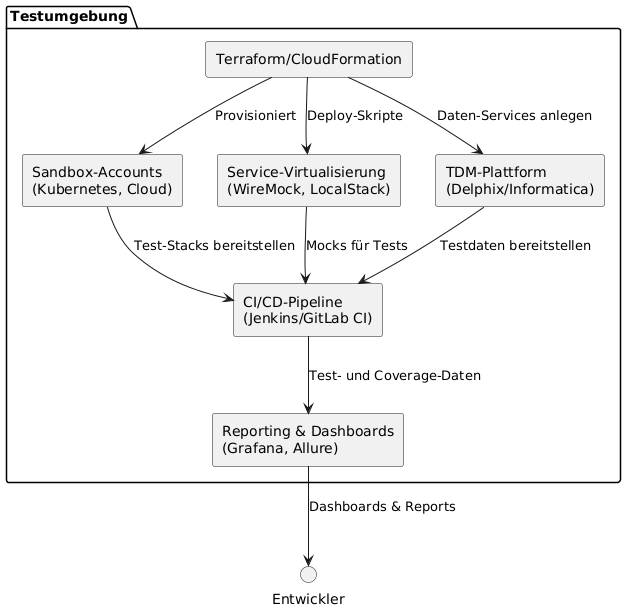
\includegraphics[width=0.8\textwidth]{fig/test_architecture_enviroment.png}
    \label{fig:architecture}
\end{figure} 
In Abbildung \ref{fig:architecture} ist unsere Testarchitektur dargestellt. Diese Architektur zeigt die verschiedenen Komponenten, die in der Testumgebung verwendet werden, einschließlich der Testautomatisierung, Service-Virtualisierung und Testdatenmanagement-Tools. Die Architektur ist so gestaltet, dass sie eine klare Trennung zwischen den verschiedenen Schichten der Testumgebung ermöglicht und gleichzeitig eine einfache Integration in die CI/CD-Pipeline gewährleistet.
\begin{itemize}
    \item \textbf{IaC}  (Terraform/CloudFormation) stellt Sandbox-Accounts, Virtualisierungs- und TDM-Komponenten bereit.
    \item \textbf{Service-Virtualisierung} (WireMock, LocalStack) simuliert externe Systeme und liefern damit isolierte Umgebungen und Mock-Services.
    \item \textbf{TDM} versorgt die Pipeline mit maskierten oder synthetischen Daten.
    \item \textbf{CI/CD-Pipeline} (Selenium, JUnit, Postman) orchestriert Tests und stellt Ergebnisse ins Reporting.
    \item \textbf{Reporting} (Allure, Grafana) aggregiert Testergebnisse und stellt sie in Dashboards dar.
\end{itemize}
\subsection{Anhang: Ablaufflow der Continuous-Testing-Pipeline}
\begin{figure}[h!]
\centering
\caption{Ablaufflow: Continuous-Testing-Pipeline}
    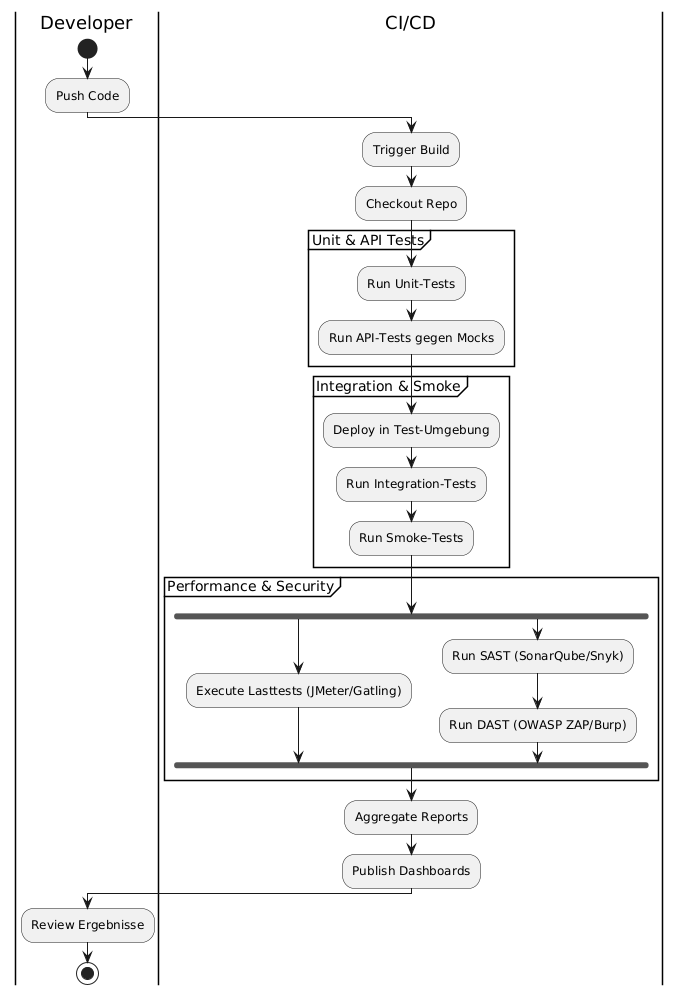
\includegraphics[width=0.8\textwidth]{fig/ablauf_pipeline.png}
    \label{fig:flow}
\end{figure} 
In Abbildung \ref{fig:flow} ist der Ablaufflow der Continuous-Testing-Pipeline dargestellt. Diese Pipeline zeigt die verschiedenen Schritte, die in der Testumgebung durchgeführt werden, nachfolgende eine kurze Beschreibung der einzelnen Schritte:
\begin{itemize}
    \item \textbf{Unit \& API Tests} laufen sofort gegen Mocks und Stubs.
    \item \textbf{Integration \& Smoke} werden in einer auf IaC bereitgestellten Testumgebung durchgeführt.
    \item \textbf{Performance \& Security} finden parallel in eigenen Phasen statt.
    \item Abschließend werden alle Reports zusammengeführt und im Dashboard veröffentlicht.
\end{itemize}
%\begin{itemize}
%    \item Welche Testtools (open source und/oder kommerziell) schlagen Sie für die Umsetzung vor für z. B.:
%    \begin{itemize}
%        \item Testautomatisierung
%        \item Performance-Testing
%        \item Service-Virtualisierung
%        \item Testdatenmanagement
%        \item Reporting \& Testmanagement
%    \end{itemize}
%\end{itemize}

%\subsection{Teamarbeit \& Rollenverteilung}
%Versucht in der Ausarbeitung die folgenden Rollen einzunehmen:
%\begin{itemize}
%    \item QA-Architekt: übergreifendes Testkonzept \& Architektur
%    \item Testanalyst: Spezifikation von Testfällen und Daten
%    \item Tool-Integrator: Toolauswahl \& CI/CD-Verknüpfung
%\end{itemize}
%Die Aufteilung ist eine Empfehlung, aber keine Pflicht.

%\subsection{Abzugebende Materialien}
%\begin{itemize}
%    \item Schriftliches Konzept (PDF, max. 6 Seiten ohne Anhang)
%    \item Architektur- oder Ablaufdiagramm(e) zur Teststrategie
%    \item Tabelle mit empfohlener Tool-Landschaft
%\end{itemize}

%\subsection{Vorgesehene Bearbeitungsdauer}
%Gesamt in etwa 5 Stunden pro Person.

%\subsection{Lernziele}
%\begin{itemize}
%    \item Eine effektive Teststrategie im Kontext von DevOps
%    \item Den Einsatz moderner Testtools konzeptionell bewerten
%    \item Risiken in komplexen Integrationslandschaften erkennen und adressieren
%    \item Testgetriebene CI/CD-Prozesse planen und visualisieren
%\end{itemize}
